\documentclass[12pt, a4paper]{report}
\usepackage[italian]{babel}
\usepackage[T1]{fontenc}
\usepackage[sfdefault]{noto}
\usepackage{graphicx}
\usepackage{multirow}
\usepackage{enumitem}
\usepackage{hyperref}
\hypersetup{pdfborder = 0 0 0 }
\usepackage{wrapfig}
\usepackage{color}
\usepackage{tabularx}
\usepackage{makecell}
\usepackage{fancyhdr}
\usepackage[font=small,labelfont=bf]{caption}
\linespread{1.3}
\textwidth=450pt\oddsidemargin=0pt
\begin{document}
\begin{titlepage}
\vspace{15mm}
\begin{center}
  
\includegraphics{Images/uniboLogo}
\end{center}
\begin{center}
{\normalsize{\bf Corso di Laurea Magistrale in Informatica}}\\
\vspace{5mm}
{\normalsize{\bf Anno Accademico 2018/2019}}\\
\vspace{20mm}
{\Large{\bf Software Architecture}}\\
\vspace{10mm}
{\Huge{\bf Kubernetes}}\\
\vspace{25mm}
\end{center}
\begin{center}
{\large{Matteo Marchesini\\0000856336\\matteo.marchesini12@studio.unibo.it}}
\end{center}
\end{titlepage}
\tableofcontents
\chapter{Descrizione del sistema}
\begin{center}
  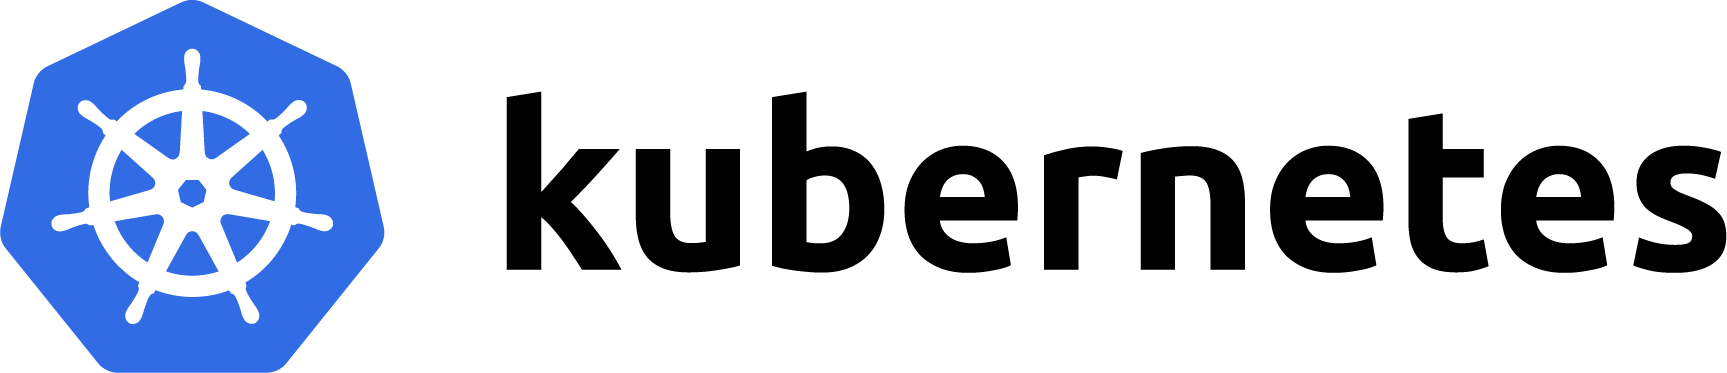
\includegraphics[scale = 0.9]{Images/kubernetesLogo}
\end{center}
Kubernetes è un sistema open source per la gestione di applicazioni containerizzate tra più host; fornisce un meccanismo per il deployment, la manutenzione e lo scaling di applicazioni. È stato inizialmente sviluppato dal team di Google, per poi passare nel 2015 sotto il controllo del \textit{Cloud Native Computing Foundation (CNCF)}, che attualmente lo supporta.\\ Al giorno d'oggi è uno dei sistemi di orchestrazione per applicazioni conteinerizzate più utilizzato in assoluto, con una vastità di utenti, partners e una comunità di development attiva. Non a caso tre dei quattro maggior providers di servizi Cloud - Microsoft, IBM e Google - offrono piattaforme di Container as a Service (CaaS) basate su Kubernetes. I servizi che Kubernetes mette a disposizione sono molteplici: fornisce un ambiente la gestione di container, microservizi e piattaforme cloud. Inoltre organizza l'infrastruttura di rete e di archiviazione per conto dell'utente.\\
In generale un sistema distribuito necessita di più componenti per il corretto funzionamento, alcune open source e altre commerciali; invece Kubernetes da solo fornisce uno scenario in cui le componenti lavorano insieme, andando così a formare un unico componente combinando la semplicità del Platform as a Service (PaaS) con la flessibilità dell'Infrastructure as a Service (IaaS).\\
L'orchestrazione di container ha avuto un profondo impatto in ogni aspetto del software development e deployment moderno; in particolare ha influenzato l'architettura del Platform as a Service, fornendo un aperto ed efficiente modello per il packaging, deployment, isolamento, scaling e rolling upgrade. Kubernetes svolgerà un ruolo cruciale nell'utilizzo di container da parte di imprese e start-up emergenti.
\\L'oggetto di questo report è di studiare tutto ciò che riguarda e circonda l'architettura di Kubernetes.
\chapter{Contesto}
\section{Scopo del sistema}
In questo capitolo verrà discusso lo scopo di Kubernetes e la sua interazione con le entità esterne, nonchè i principali casi d'uso. \\
Kubernetes, come introdotto nel Capitolo 1, è un sistema di orchestrazione di container e per questo motivo si occupa principalmente di \textbf{deployment}, \textbf{scaling} e \textbf{management} di applicazioni containerizzate. Di seguito viene definito ognuno di questi tasks:
\begin{itemize}
\item \textbf{Deployment}: gestisce la distribuzione di applicazioni assegnando ai nodi del cluster ciascuna istanza dell'applicazione. Il deployment in Kubernetes può essere eseguito in una varietà di ambienti con pattern differenti, ed esistono appunto diversi modelli, quali:
\begin{itemize}
  \item Container as a Service (CaaS);
  \item Public Cloud - Infrastructure as a Service (IaaS);
  \item Utilizzo on-premises all'interno di data center;
  \item Deployment ibrido
\end{itemize}
\item \textbf{Scaling}: permette di ridimensionare l'applicazione a seconda delle esigenze dell'utente, andando a modificare le dimensioni del cluster e il numero di repliche dei pod. Un \textbf{pod} è il più piccolo oggetto deployabile nel modello a oggetti di Kubernetes e può incapsulare un singolo container o più container che necessitano di lavorare insieme.
\item \textbf{Management}: fornisce un'interfaccia per la gestione dei cluster e delle applicazioni containerizzate. Un cluster di Kubernetes viene ospitato e gestito da un venditore commerciale, quali ad esempio Google Container Engine (GKE), Amazon EC2 Container Service e Azure Container Service di Microsoft, che offrono servizi di CaaS nel cloud pubblico. Molti utenti hanno iniziato ad usare Kubernetes attraverso Google Container Engine, essendo uno dei primi servizi di gestione di Kubernetes nel mercato.
\end{itemize}
\section{Entità esterne}
Nella figura seguente è espresso il \textit{system context diagram} di Kubernetes, che definisce le relazioni tra esso e le entità esterne.
\begin{center}
  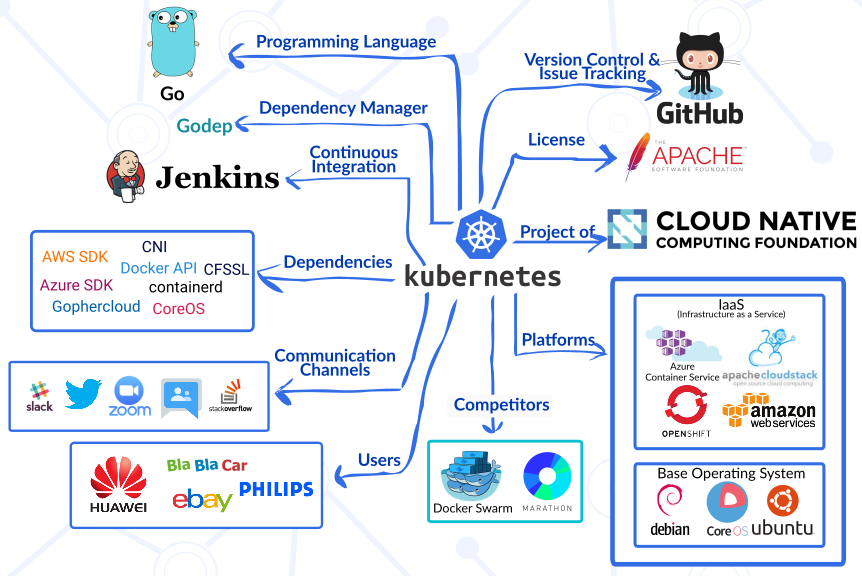
\includegraphics[scale = 0.6]{Images/ContextModelDiagram}
\end{center}
Le entità di maggior rilievo all'interno del diagramma e che verranno analizzate in seguito sono gli stakeholders, il development, le piattaforme e i concorrenti.
\subsection{Stakeholders}
Per poter comprendere al meglio il concetto di stakeholder all'interno di un progetto così grande come quello di Kubernetes, è necessario introdurre il \textbf{Cloud Native Computing Foundation} (CNCF).\\
CNCF è nato nel 2015 da un accordo tra Google e la Linux Foundation con l'annuncio di Kubernetes 1.0, considerato il progetto principale. Da li in poi molte industrie del cloud computing si sono unite a CNCF per incubare, sviluppare e mantenere un ecosistema di progetti cloud sotto una visione comune e condivisa. I membri di CNCF sono divisi per categorie, quali Platinum, Gold, Silver, End-User, accademici e no-profit. Tra i membri Platinum abbiamo Google, Docker, IBM, Cisco e Oracle.\\
Oltre all'organizzazione CNCF, Kubernetes attrae migliaia di contributori che coordinano i loro sforzi attraverso piattaforme online, quali GitHub, Slack e StackOverflow (fornitori). Gli Special Interest Groups (SIG) si occupano dello sviluppo di Kubernetes, in particolare dell'architettura, del product management e del testing, nonchè di implementazione specifiche per fornitori di servizi come AWS e Azure.
\subsubsection{Griglia Power/Interest}
Nella seguente immagine è raffigurata la griglia o matrice \textit{power/interest} che divide gli stakeholders in quattro categorie:
\begin{itemize}
  \item \textbf{Alta potenza e alto interesse}: la massima potenza suoi progetti di Kubernetes la detiene il consiglio d'amministrazione di CNCF che ne gestisce il budget, seguito poi da CNCF TOC (Technical Oversight Committee), che ha il compito di aggiungere e rimuovere progetti come Kubernetes. Inoltre anche l'architettura SIG è fondamentale in quanto decide il futuro del progetto.
  \item \textbf{Alta potenza e basso interesse}: il CNCF Marketing Committee, derivato dal consiglio di amministrazione di CNCF, cura il brand del progetto e altre attività legate al business.
  \item \textbf{Bassa potenza e alto interesse}: rispetto agli stakeholder con grande potere su Kubernetes, il CNCF end user TAB, lo staff di provider di piattaforme/servizi, Test SIG e la comunità di sviluppatori generali di Kubernetes dipendono dal continuo sviluppo del progetto, e questo comporta un alto interesse.
  \item \textbf{Bassa potenza e basso interesse}: le piattaforme di coordinamento, quali GitHub, hanno scarso potere ed interesse per il progetto, in quanto altre piattaforme potrebbero avere uno scopo simile se non fossero prese in considerazione.
\end{itemize}
\begin{center}
  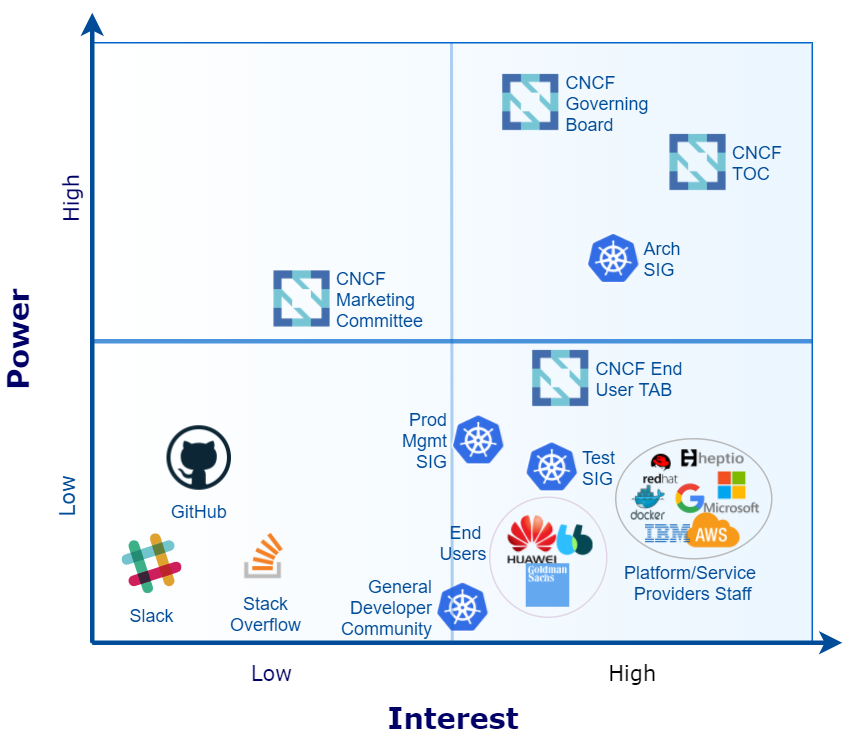
\includegraphics[scale = 0.45]{Images/power-interest}
\end{center}
\subsection{Development}
Il principale linguaggio con cui Kubernetes è sviluppato è \textbf{Go}, un linguaggio open-source progettato da tre ingegneri di Google, ma nonostante ciò possiede dipendenze da varie librerie esterne, quali Amazon Web Services SDK (AWS), Docker API, Azure SDK,  Container Network Interface (CNI), e Gophercloud. Inoltre Kubernetes si affida a Jenkins per la Continuous Integration.
\subsection{Piattaforme}
Kubernetes essendo una piattaforma cloud è compatibile con diverci providers a seconda delle necessità e dell'utilizzo. Di seguito sono riportate alcune soluzioni differenti a seconda del pattern di utilizzo.
\subsubsection{Container Management, soluzioni in locale e PaaS}
\begin{table}[ht]
  \small
  \begin{center}
  \begin{tabularx}{\textwidth}{|lr|}
    \hline
    \textbf{Prodotto} (compagnia) & \textbf{Categoria}\\
    \hline
    \textbf{AppsCode} (AppsCode)&Hosted, PaaS\\
    \multicolumn{2}{|X|}{\textit{È una piattaforma integrata per il deployment, testing e coding di app containerizzate. Permette il deployment su Google Cloud Platform e AWS.}}\\
    \hline
    \textbf{Cloud Container Engine} (Huawei)&CaaS\\
    \multicolumn{2}{|X|}{\textit{Servizio di containerizzazione scalabile ad alte prestazioni basato su Kubernetes}}\\
    \hline
    \textbf{Giant Swarm} (Giant Swarm)&Hosted, on-premises\\
    \multicolumn{2}{|X|}{\textit{Una soluzione creare, distribuire e gestire servizi containerizzati con Kubernetes come componente principale}}\\
    \hline
    \textbf{Google Container Engine} (Google)&CaaS\\
    \multicolumn{2}{|X|}{\textit{Google Container Engine è un sistema di gestione e orchestrazione dei cluster che consente agli utenti di eseguire container sulla piattaforma Cloud di Google}}\\
    \hline
    \textbf{OpenShift Container Platform} (RedHat)&PaaS, on-premises\\
    \multicolumn{2}{|X|}{\textit{Una piattaforma di applicazioni per container che può estendersi su più infrastrutture. È costruito usando la tecnologia Docker e Kubernetes.}}\\
    \hline
  \end{tabularx}
  \end{center}
\end{table}

\begin{table}[ht]
\small
\centering
\begin{tabularx}{\textwidth}{|lr|}
\hline
\textbf{OpenShift Online} (RedHat)&Hosted\\
\multicolumn{2}{|X|}{\textit{Versione hosted di OpenShift. Il funzionamento è il medesimo a quello di OpenShift Container Platform}}\\
\hline
\textbf{Platform9 Managed Kubernetes for Docker} (Platform9)&Hosted, on-premises\\
\multicolumn{2}{|X|}{\textit{I clienti possono utilizzare il singolo pannello di Platform 9 per orchestrare e gestire i container insieme alle macchine virtuali. In pratica, è possibile orchestrare le VM utilizzando OpenStack e/o Kubernetes}}\\
\hline
\end{tabularx}
\end{table}

\subsubsection{Tools per deployment e controllo di clusters Kubernetes}
\begin{table}[ht]
\small
\centering
\begin{tabularx}{\textwidth}{|lr|}
\hline
\textbf{Prodotto} (compagnia) & \textbf{Categoria}\\
\hline
\textbf{AppFormix} (AppFormix)&Monitoring\\
\multicolumn{2}{|X|}{\textit{Fornisce metriche e analisi per i container. Gli utenti possono gestire avvisi, o regole di orchestrazione per singoli pods o container. La dashboard può essere ulteriormente personalizzata e mappata nei propri progetti}}\\
\hline
\textbf{Bootkube} (CoreOS)&Deploy\\
\multicolumn{2}{|X|}{\textit{Uno strumento di supporto per l'avvio di cluster Kubernetes autogestiti.}}\\
\hline
\textbf{ElasticBox ElasticKube} (CenturyLink)&Deploy\\
\multicolumn{2}{|X|}{\textit{Un servizio per pipeline di CI/CD, per la configurazione di tools di management e per il deployment di applicazioni cloud. Include ElasticKube, una piattaforma open source per Kubernetes che promuove il self-service per le applicazioni containerizzate.}}\\
\hline
\textbf{Kubernetes Dashboard} (Cloud Native Computing Foundation)&Monitor\\
\multicolumn{2}{|X|}{\textit{Fornisce un'interfaccia utente basata sul Web per cluster Kubernetes. Consente agli utenti di gestire le applicazioni in esecuzione nel cluster nonché di gestire il cluster stesso.}}\\
\hline
\textbf{Minikube} (Cloud Native Computing Foundation)&Deploy\\
\multicolumn{2}{|X|}{\textit{Minikube è un tool che permette di eseguie in locale Kubernetes, semplicemente eseguendolo all'interno di una VM del proprio pc. }}\\
\hline
\end{tabularx}
\end{table}
\newpage
\subsubsection{Tool per integration}
\begin{table}[ht]
\small
\centering
\begin{tabularx}{\textwidth}{|l|}
\hline
\textbf{Prodotto} (compagnia) \\
\hline
\textbf{Apprenda} (Apprenda)\\
\multicolumn{1}{|X|}{\textit{Fornisce PaaS private per le aziende che supportano l'hosting di container}}\\
\hline
\textbf{Crunchy PostgreSQLContainer Suite} (Crunchy Data)\\
\multicolumn{1}{|X|}{\textit{Un set di container Docker e servizi Kubernetes "preconfezionato"; il Crunchy Container Suite permette ai team di eseguire e gestire PostgreSQL su ambienti basati su Kubernetes}}\\
\hline
\textbf{fabric8} (Red Hat)\\
\multicolumn{1}{|X|}{\textit{Una piattaforma open-source per il DevOps e integrazione costruita con un set di microservizi eseguiti su Kubernetes e OpenShift V3. La sua continuos delivery è basata su Jenkins, Nexus e SonarQube}}\\
\hline
\textbf{Kubeflix} (Red Hat)\\
\multicolumn{1}{|X|}{\textit{Integrazione di Kubernetes con i componenti open source di Netflix, quali Hystrix, Turbine e Ribbon}}\\
\hline
\textbf{NetScaler CPX} (Citrix)\\
\multicolumn{1}{|X|}{\textit{Sistema di bialnciamento della containerizzazione in Docker che può essere supportata on-premises o in ambienti multi-cloud. NetScaler CPX si integra con Kubernetes al fine di bilanciare applicazione containerizzate all'interno di cluster. Nell'ambiente di Kubernetes, NetScaler CPX rimpiazza kube-proxy nei minion e bilancia il carico nei pod. }}\\
\hline
\end{tabularx}
\end{table}
\newpage
\subsection{Concorrenti}
Tra i tool concorrenti a Kubernetes che offrono un servizio di orchestrazione di container abbiamo \textbf{Docker Swarm} e \textbf{Marathon}. Marathon è una piattaforma di orchestrazione di applicazioni e servizi per Apache Mesos.\\
Docker Swarm invece, che è integrato in Docker come \textit{Swarm Mode}, è un orchestratore per i container Docker. Confrontando Docker Swarm con Kubernetes, emerge che quest'ultimo è un tool molto più efficiente, in quanto offre una maggiore scalabilità e automazione. Inoltre Kubernetes possiede delle proprie librerie per il monitoraggio e i logging; ciò viene a mancare in Docker Swarm, che deve ricorrere ad applicazioni di terze parti per sopperire a queste features.
Kubernetes supera i vincoli imposti da Docker e Docker API per il deployment, e per questo è maggiormente utilizzato. In Kubernetes se un nodo fallisce, esso viene rimpiazzato così velocemente da non accorgersi, a meno che non si esegua una dettagliata risoluzione dei problemi.
\chapter{Drivers architetturali}
Kubernetes, come si può capire dal capitolo precedente, è progettato secondo i principi di scalabilità, disponibilità e sicurezza, nonchè fornisce una distribuzione del carico di lavoro tra le risorse disponibili. Questo capitolo metterà in evidenza alcuni dei requisiti non funzionali di Kubernetes.
\section{Scalabilità}
Le applicazioni sono eseguite in Kubernetes come microservizi. Tali microservizi sono composti da più container raggruppati in \textbf{pods}. Ciascun container è progettato per eseguire solamente un unico task.\\
I pods possono essere composti da container con o senza stato (stateless/stateful). I pods senza stato possono essere scalati facilmente quando necessario anche attraverso l'auto-scaling dinamico.\\
Dalla versione 1.4 Kubernetes supporta l'auto-scaling orizzontale dei pod, che scala autmaticamente il numero di pod in repliche controllate basate sull'utilizzo della CPU. La versione di Kubernetes ospitata da Google Cloud supporta l'auto-scaling di cluster. Quando un nuovo pod viene scalato tra tutti i nodi disponibili, Kubernetes coordina l'infrastruttura sottostante per far si che ulteriori nodi vengano aggiunti al cluster. \\
  \begin{center}
  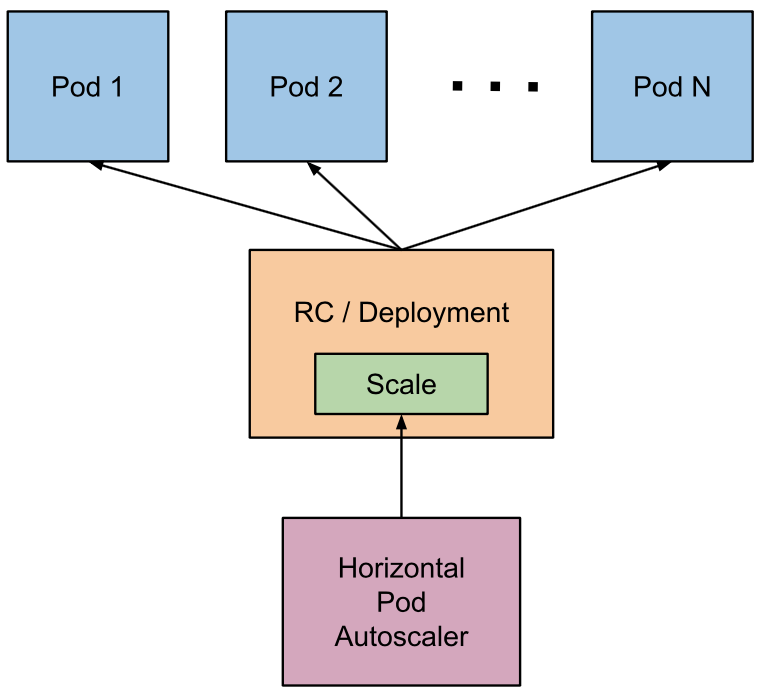
\includegraphics[scale = 0.7]{Images/horizontal-pod-autoscaler}
  \captionof{figure}{Autoscaling orizzontale di un pod}
  \end{center}
L'auto-scaling orizzontale è implementato come un loop di controllo, in cui periodicamente (con un valore predefinito di 30 secondi) il controller manager interroga l'utilizzo delle risorse rispetto alle metriche specificate in ciascuna definizione di \textit{HorizontalPodAutoscaler}.
Nello specifico, il controller manager ottiene le metriche (ad esempio l'utilizzo di CPU) attraverso l'API apposita per le metriche; quindi se è settato un valore target di utilizzo, il controller calcola il valore di utilizzo come percentuale delle richieste alle risorse equivalenti contenute nei container di ciascun pod. Se invece è impostato un valore grezzo, il controller utilizza direttamente tale valore. Il controller quindi assume o la media di utilizzo o il valore grezzo, per produrre poi un rapporto usato per scalare il numero di repliche desiderate. Da sottolineare il fatto che se alcuni container all'interno dei pods non hanno il set di richieste di risorse rilevanti, l'utilizzo di CPU per quel dato pod non verrà definito e l'autoscaler non intraprenderà alcuna azione per tale metrica.\\
Kubernetes supporta inolte lo scaling di applicazioni stateless come i cluster Cassandra e i set di repliche MongoDB, ovvero più in generale di workloads persistenti, quali i database NoSQL e i database relazionali (RDBMS).
\section{Disponibilità}
In kubernetes i carichi di lavoro richiedono la disponibilità sia a livello di infrastruttra che applicazione. Ad esempio, nei cluster a larga scala, tutto è soggetto ai guasti, il che rende necessaria un'elevata disponibilità per la produzione dei workloads.
Mentre la maggior parte dei motori di orchestrazione di container offrono la disponibilità di applicazioni, Kubernetes è progettato per affrontare la disponibilità sia di applicazioni che di infrastrutture.\\
Per quanto riguarda il fronte applicazione, Kubernetes assicura un alta disponibilità per mezzo di \textit{ReplicaSet}, \textit{Replication Controller} e \textit{StatefulSets}. Un ReplicaSet garantisce che un numero specificato di repliche di pod siano in esecuzione in qualsiasi momento, e lo stesso vale per i Replication Controller, con l'unica differenza che quest'ultimo supporta solo il selettore di uguaglianza, mentre ReplicaSet supporta il selettore basato sul set.\\
Quindi l'utilizzatore di Kubernetes può dichiarare il numero minimo di pods che devono essere eseguiti in un dato istante di tempo. Se un container o un pod si arresta in modo anomalo a causa di un errore, la policy dichiarativa può riportare il deployment alla configurazione desiderata.\\
Analizzando la disponibilità rispetto all'infrastruttura, Kubernetes supporta un'ampia gamma di back-end di archiviazione, quali file systems distribuiti, come il file systems di rete (\textbf{NFS}) e \textbf{GlusterFS}, gli storage persistente a livello di blocco, come \textbf{Amazon Elastic Block Store} (EBS) e Google Compute Engine, e infine container di storage come \textbf{Flocker}, un open-source Container Data Volume Manager per le applicazioni in Docker. L'aggiunta di un livello di archiviazione affidabile e disponibile a Kubernetes garantisce un'elevata disponibilità di workloads statici. Ogni componente del cluster di Kubernetes - etcd, API server, nodi - può essere configurato per garantire un alta disponibilità. Le applicazioni hanno quindi il vantaggio di usufruire di un bilanciamento del carico di lavoro e di checks di controllo per garantire disponibilità.
\section{Sicurezza}
La sicurezza in Kubernetes è configurata su più livelli. Gli endpoints dell'API sono protetti tramite Transport Layes Security (\textbf{TLS}), che garantisce l'autenticazione dell'utente utilizzando il meccanismo di autenticazione più sicuro disponibile. I cluster di Kubernetes hanno due categorie di utenti:
\begin{itemize}
  \item Service account, gestiti direttamente da Kubernetes;
  \item Utenti normali, che si suppone essere gestiti da un servizio indipendente.
\end{itemize}
I service account gestiti da Kubernetes sono creati in automatico dall'API server. Ciascuna operazione che gestisce un processo in esecuzione all'interno di un cluster deve essere avviata da un utente autenticato; questo meccanismo garantisce la sicurezza del cluster.\\
Le applicazioni eseguite all'interno di un cluster Kubernetes possono beneficiare del concetto di \textit{segreti} per un accesso sicuro ai dati. Un \textbf{segreto} è un oggetto Kubernetes che contiene una piccola quantità di dati sensibili, come password, token o chiave, che riduce il rischio di esposizione accidentale dei dati. Gli username e le password sono codificati in base64 prima di essere memorizzati all'interno del cluster Kubernetes. I pod possono accedere al segreto in fase di runtime tramite i volumi montati o le variabili d'ambiente.\\
Per permettere o limitare il traffico di rete ai pods, le politiche di rete possono essere applicate al deployment. Una policy di rete è una specifica di come i gruppi di pod possono comunicare tra loro e con altri endpoint di rete. Ciò può risultare utile in un deployment a più livelli per oscurare i pods in modo da non essere esposti ad altre applicazioni.
\begin{center}
  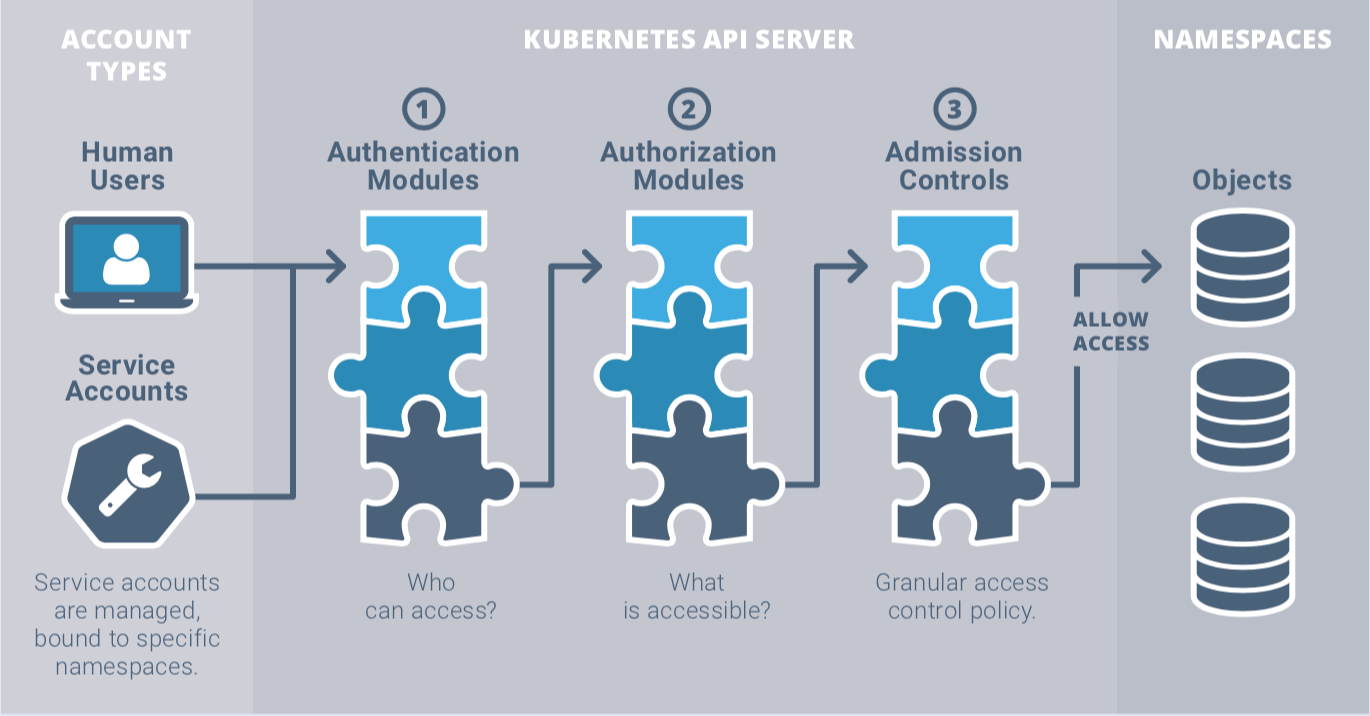
\includegraphics[scale = 0.5]{Images/Kubernetes-auth}\\
\captionof{figure}{Utilizzo dei moduli di autenticazione, autorizzazione e Admission Control per controllare l'accesso API in Kubernetes.}
\end{center}
\section{Portabilità}
Kubernetes è progettato per offrire una libertà di scelta rispetto alla scelta del sistema operativo da utilizzare, all'esecuzione dei container, all'architettura del processore, alle piattaforme cloud e al PaaS.\\
Infatti un cluster Kubernetes può essere configurato nelle principali distribuzioni Linux, quali CentOS, CoreOS, Debian, Fedora, Red Hat Linux e Ubuntu. Può essere eseguito in locale oppure in piattaforme cloud, come AWS, Azure e Google Cloud; su ambienti virtualizzati basati su KVM e vSphere. Gli utenti possono lanciare container in Docker o rkt runtimes, e nuovi container possono essere lanciati anche a tempo di esecuzione. \\
Inoltre attraverso la \textit{federation} è anche possibile combinare cluster eseguiti tra più cloud provider differenti e in locale. Ciò porta le funzionalità del cloud ibrido ai workloads containerizzati. In questo modo i clienti possono facilmente spostare i carichi di lavoro da un target di deployment all'altro.
\chapter{Struttura architetturale}
Al giorno d'oggi le applicazioni conteinerizzate necessitano di un'infrastruttura sufficientemente solida per far fronte alle esigenze del clustering e allo stress dell'orchestrazione dinamica. Tale infrastruttura deve poter permettere lo scheduling, il monitoraggio, l'aggiornamento e il reallocamento dei container tra i vari host. Deve essere in grado di trattare la computazione, l'archiviazione e le primitive di rete sottostanti come un pool di risorse. Ogni carico di lavoro containerizzato dovrebbe essere in grado di sfruttare le risorse a esso esposte, inclusi CPU, unità di archiviazione e reti.
\begin{center}
  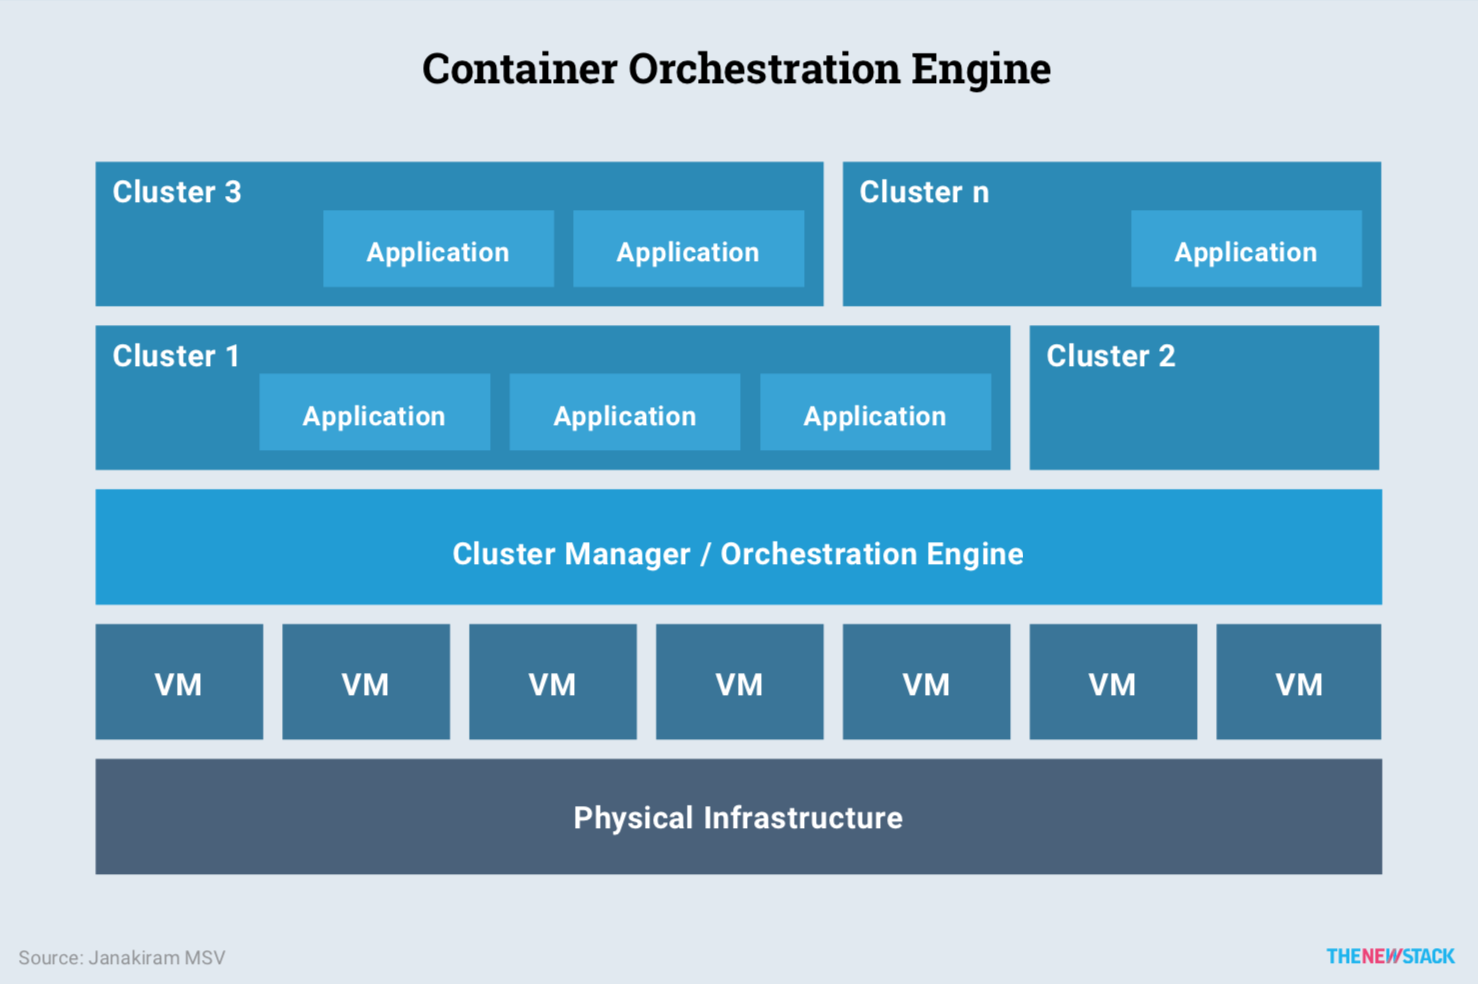
\includegraphics[scale=0.4]{Images/Kubernetes-overview}
  \captionof{figure}{I livelli del sistema, da un punto di vista di orchestrazione dei container}
\end{center}
Kubernetes è un gestore open source di cluster che astrae l'infrastruttura fisica sottostante, semplificando l'esecuzione di applicazioni containerizzate su larga scala. Un'applicazione, gestita per l'intero ciclo di vita da Kubernetes, è composta da un set di container raccolti e coordinati in una singola unità. Un efficiente livello di gestione del cluster permette a Kubernetes di poter disaccopiare efficacemente l'applicazione dall'infrastruttura di supporto, come mostrato in figura 4.1. Una volta che l'infrastruttura di Kubernetes è stata configurata i team DevOps possono concentrarsi sulla gestione dei carichi di lavoro distribuiti piuttosto che gestire il pool di risorse sottostanti.
L'API di Kubernetes può essere utilizzata per creare i componenti che fungono da blocchi fondamentali, o primitive, di microservizi. Questi componenti sono autonomi, il che significa che esistono indipendentemente dagli altri componenti.
\section{Pod}
Un pod è una collezione di uno o più container che funge da unità principale di Kubernetes per la gestione del carico di lavoro, fungendo da "confine logico" per i container che condividono contesto e risorse. Raggruppare container correlati in pod fa fronte alle sfide configurazionali introdotte quando la containerizzazione ha sostituito la virtualizzazione di prima generazione, rendendo possibile l'esecuzione di più processi dipendenti.\\In fase di runtime, i pod possono essere ridimensionati creando set di repliche, che garantiscono che la distribuzione esegua sempre il numero desiderato di pod. Come già anticipato ogni pod è una raccolta di più container e per comunicare tra loro utilizzano le remote procedure calls (RPC), condividendo lo stack di archiviazione e di rete.\\
Negli scenari in cui i container devono essere accoppiati e co-localizzati, ad esempio un contenitore del server Web e un contenitore della cache, possono essere facilmente raccolti in un singolo pod. Un pod può essere scalato manualmente o tramite una feature chiamata Horizontal Pod Autoscaling (HPA).\\
Attraverso questo metodo il numero dei container al'interno di un pod viene aumentato proporzionalmente.
\begin{center}
  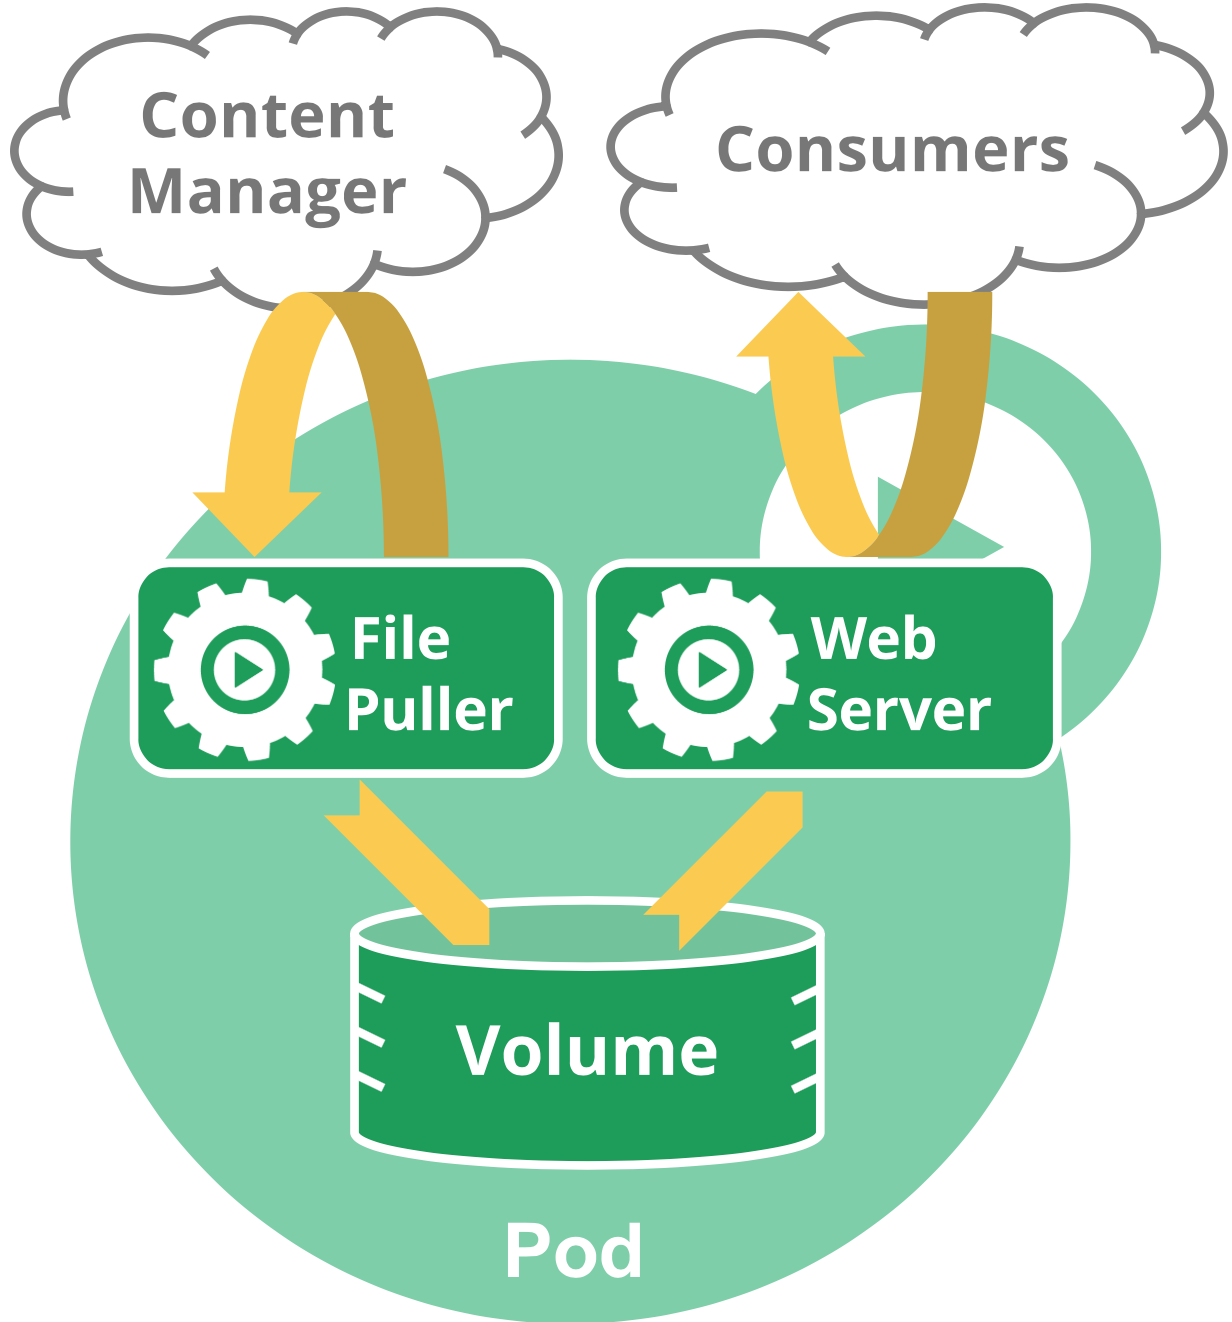
\includegraphics[scale=0.4]{Images/Kubernetes-pod}
  \captionof{figure}{Un pod multi-container che contiene un file puller e un server Web che utilizza un volume persistente per l'archiviazione condivisa tra container}
\end{center}
I Pods consentono inoltre un separazione funzionale tra development e deployment. Mentre gli sviluppatori si concentrano sul loro codice, gli operatori possono concentrarsi su una visione più ampia di come i container possono essere uniti insieme in un'unità funzionale. Il risultato ottenuto è una quantità ottimale di portabilità, dal momento in cui un pod non è altro che la rappresentazione di più immagini di container gestiti insieme.
\section{Service (SOA)}
Kubernetes, come la maggior parte dei sistemi distribuiti, è progettato secondo un'architettura orientata ai microservizi (\textbf{SOA}). In generale in questo tipo di architettura, ogni servizio ha un proprio contesto funzionale distinto e l'interazione con qualsiasi cosa al di fuori di tale contesto avviene tramite un'interfaccia astratta, in genere l'API di un altro servizio pubblico.\\
\\
Nel caso di Kubernetes, un singolo pod o un ReplicaSet può essere esposto a client interni o esterni attraverso servizi, che associano un set di pod secondo un criterio specifico. Quando viene creato un pod, viene assegnato un indirizzo IP accessibile solo all'interno del cluster. Ma non vi è alcuna garanzia che l'indirizzo IP del pod rimarrà invariato per tutto il suo ciclo di vita. Kubernetes può reallocare o re-instanziare i pod in fase di runtime, creando un nuovo indirizzo IP per il pod. Per compensare questa incertezza, i servizi assicurano che il traffico sia sempre indirizzato al pod appropriato all'interno del cluster, indipendentemente dal nodo su cui è pianificato.  Ogni servizio espone un indirizzo IP e può anche esporre un endpoint DNS, entrambi i quali non cambieranno mai. I consumatori interni o esterni che necessitano di comunicare con un set di pod utilizzeranno l'indirizzo IP del servizio o il suo endpoint DNS più noto. In questo modo, il servizio funge da colla per il collegamento di pod con altri pod.
\\
In Kubernetes qualsiasi oggetto API, incluso un nodo o un pod, può avere coppie chiave-valore ad esso associate o metadati aggiuntivi per identificare e raggruppare oggetti che condividono un attributo o una proprietà comune. Kubernetes si riferisce a queste coppie chiave-valore come etichette, in inglese \textbf{"labels"}. \\
Un \textbf{selettore} è un tipo di criterio utilizzato per interrogare gli oggetti di Kubernetes che corrispondono a un valore di label. QUesta potente tecnica consente di avere un basso accoppiamento tra oggetti. Inoltre possono essere creati nuovi oggetti che corrispondono al valore indicato dal selettore. Labels e selettori formano il meccanismo principale di Kubernetes per identificare i componenti ai quali si applica un'operazione.\\
Un \textbf{ReplicaSet} si basa su etichette e selettori per determinare quali pods saranno scalati. In fase di runtime i pod possono essere scalati attraerso i ReplicaSet garantendo così che ogni deployment abbia sempre il numero desiderato di pods. Ogni pod la cui etichetta corrisponde al selettore definito dal servizio verrà esposto il suo endpoint. Quando un'operazione di scaling viene avviata da un set di repliche, i nuovi pod creati da tale operazione inizieranno immediatamente a ricevere il traffico. Un servizio fornisce quindi il bilanciamento del carico di base instradando il traffico tra i pod di corrispondenza.
\\
Questa architettura fornisce un meccanismo flessibile e liberamente accoppiato per l'individuazione dei servizi. Infatti la decostruzione di un sistema in un insieme di servizi complementari disaccoppia le operazioni tra le varie parti. Questa astrazione aiuta a stabilire chiare relazioni tra i servizi, il suo ambiente sottostante e i consumatori di quel servizio.\\
Creare chiare delineazioni può aiutare a isolare i problemi, ma permette inoltre di scalare ciascun servizio indipendentemente dagli altri. Questo tipo di progettazione orientata ai servizi è molto simile alla programmazione orientata agli oggetti.
\begin{center}
  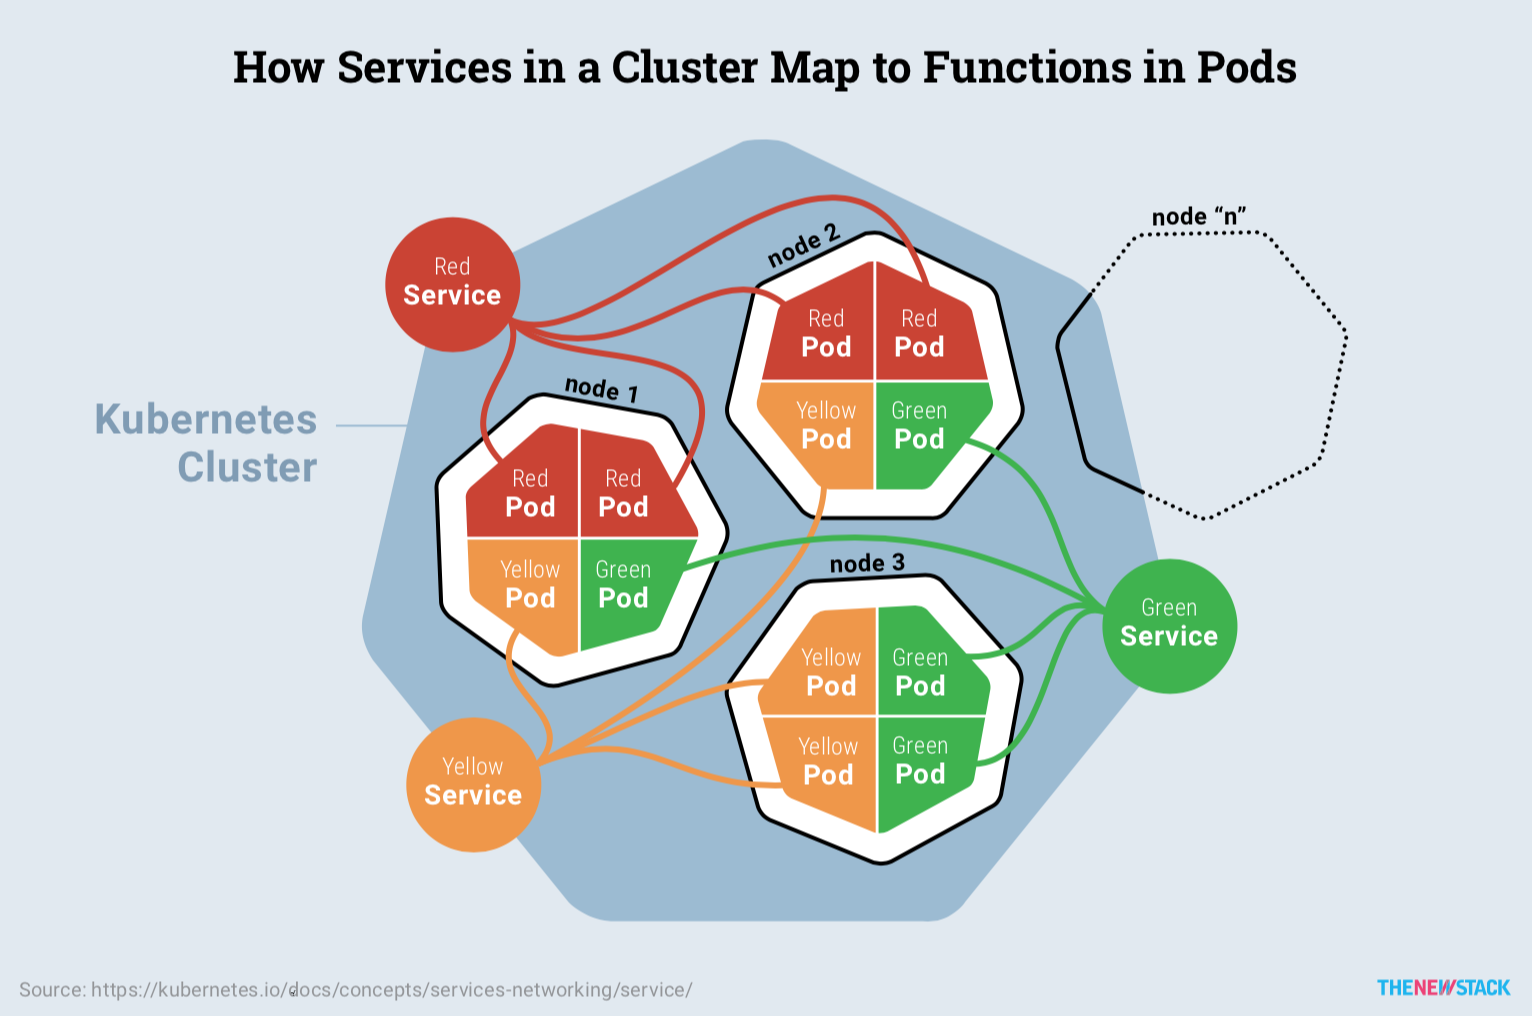
\includegraphics[scale=0.6]{Images/Kubernetes-service}
  \captionof{figure}{I servizi in Kubernetes}
\end{center}
La figura 4.3 mostra la funzionalità dei servizi all'interno di un cluster Kubernetes. Sono presenti tre tipi di pod, distinti dai colori giallo, verde, rosso. Un replication controller ha scalato tali pod per eseguire istanze su tutti i nodi disponibili. Ogni classe di pod è esposto ai clients attraverso un servizio, rappresentato dal cerchio colorato.\\
Supponendo che ogni pod abbia una label della forma \textit{color=value}, il suo servizio associato dovrebbe avere un selettore che lo abbini.\\ \\
Quando un client raggiunge il servizio rosso, la richiesta viene inoltrata a un qualsiasi pod che abbia la label \textit{color=red}. Se viene aggiunto un nuovo pod in seguito ad uno scaling, esso viene immediatamente rilevato dal servizio, in virtù della label e del selettore corrispondente.\\ \\
In Kubernetes i servizi possono essere configurati per esporre pods a client interni o esterni. Un servizio esposto internamente è raggiungibile attraverso l'indirizzo \textbf{ClusterIP}, ovvero l'indirizzo del cluster. Questi tipi di servizio sono ad esempio i pods Database, che non necessitano di essere esposti esternamente. Invece quando un servizio necessita di essere raggiunto dall'esterno, è necessario esporre una porta specifica in ciascun nodo, chiamata \textbf{NodePort}. \\
Negli ambienti cloud pubblici, Kubernetes può eseguire il servizio di bilanciamento del carico configurato automaticamente per il routing del traffico ai suoi nodi.
\chapter{Comportamento}
Kubernetes, come la maggior parte delle piattaforme distribuite, è composto da almeno un nodo master e nodi di lavoro multipli. In alcuni casi, per garantire alta disponibilità, i nodi master possono essere anche più di uno. Nella seguente immagine viene rappresentata l'architettura di Kubernetes con tutte le sue componenti, che verranno analizzate singolarmente.
\begin{center}
  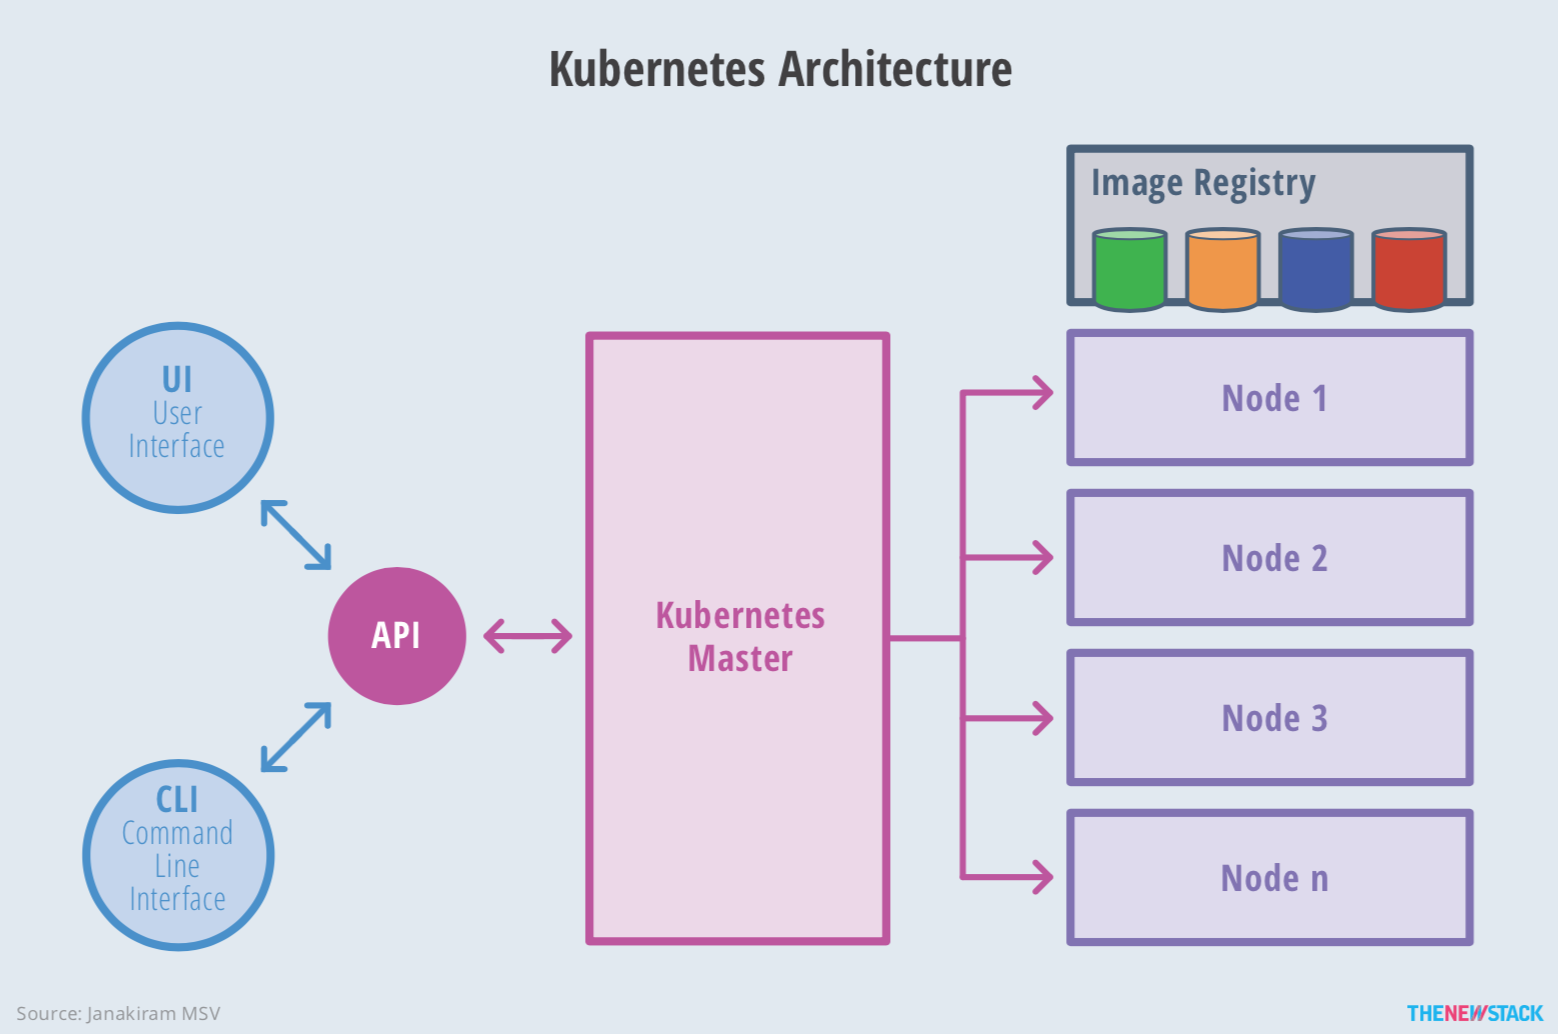
\includegraphics[scale=0.5]{Images/Kubernetes-architecture}
  \captionof{figure}{Componenti dell'architettura di Kubernetes}
\end{center}
\section{Nodo Master}
Il nodo \textbf{master} è responsabile per l'esposizione dell' API (application program interface), per la pianificazione del deployment e la gestione dell'intero cluster. Attraverso l'esposizione dell'API fornisce all'utente un'interfaccia per poter interagire con il sistema. Concettualmente, all'interno del nodo master non ci dovrebbero essere container in esecuzione.\\
La definizione degli oggetti in Kubernetes, così come i pods, i Replica sets e i servizi sono un compito del nodo master. Sono progettati per essere liberamente accoppiati, estendibili e adattabili a un'ampia varietà di carichi di lavoro. L'API fornisce questa estensibilità ai componenti interni, nonché estensioni e container in esecuzione su Kubernetes.
\begin{center}
  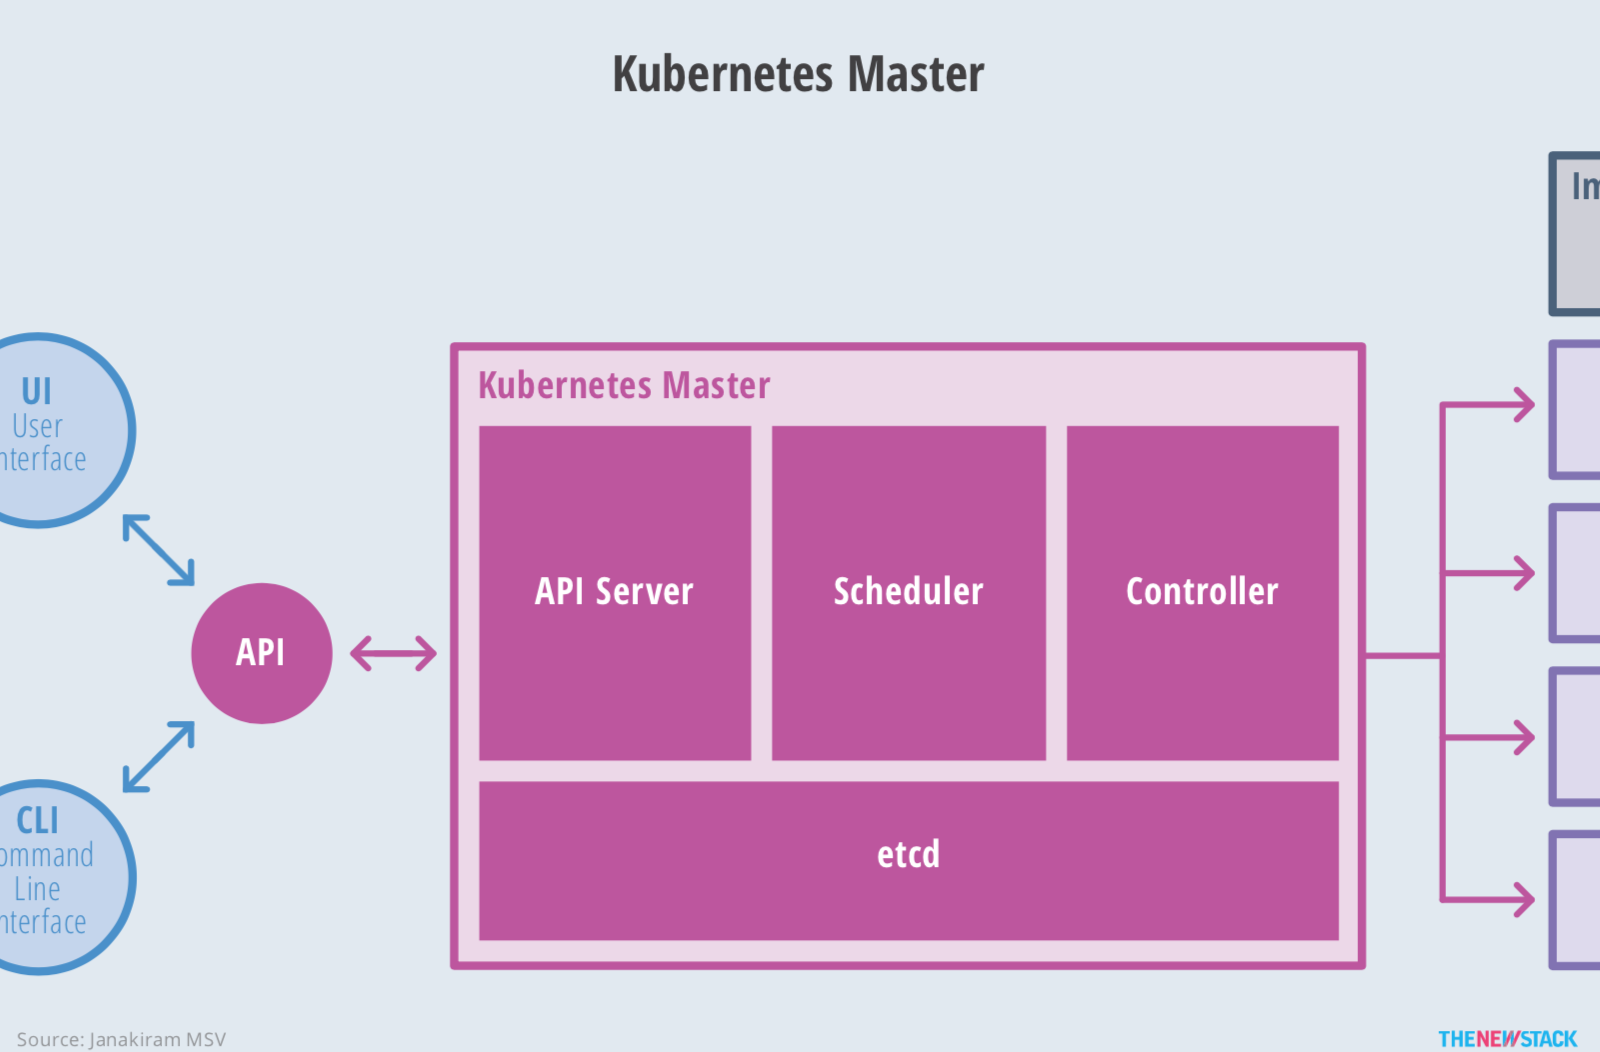
\includegraphics[scale=0.5]{Images/Kubernetes-master}
  \captionof{figure}{Componenti del nodo master}
\end{center}
Come osservabile dalla figura 4.2, il nodo master si compone di più elementi:
\begin{itemize}
  \item \textbf{kube-apiserver}: Il server API espone l'API di Kubernetes tramite JSON su HTTP, fornendo l'interfaccia REST per gli endpoint interni ed esterni dell'orchestratore per interagire con altri componenti del sistema. Impiega etcd-storage come componente di archiviazione persistente. La CLI, l'interfaccia utente web o un altro strumento possono inviare una richiesta al server API. Il server elabora e convalida la richiesta, quindi aggiorna lo stato degli oggetti API in etcd e infine istruisce il servizio appropriato per eseguirla. Ciò consente ai client di configurare carichi di lavoro e container tra i nodi worker.
  \item \textbf{etcd-storage}: etcd è un database di CoreOS chiave-valore, distribuito e open-source, nonchè persistente e leggero. Agisce come unica fonte per tutti i componenti del cluster di Kubernetes, infatti altri componenti e servizi guardano le modifiche a etcd per mantenere lo stato desiderato di un'applicazione. Il nodo master utilizza \textit{etcd} per memorizzare i suoi stati, ad esempio i job pianificati, creati e dstribuiti; dettagli e stato dei pod; informazioni sulle repliche, e altro.
  \item \textbf{kube-scheduler}: lo scheduler è responsabile di trovare un nodo corretto al quale assegnare un pod o un servizio, in base ad alcuni vincoli, ad esempio cerca di bilanciare l'utilizzo delle risorse tra i vari nodi e assicura che i pod si trovino su nodi che abbiano risorse libere a sufficienza.
  \item \textbf{controller-manager}: il controller manager, o semplicemente controller, è un processo che al suo interno incapsula vari controllers. In kubernetes, il controller è identificato come un loop di controllo che periodicamente controlla lo stato del cluster attraverso \textit{kube-apiserver} ed esegue le opportune modifiche per far si che il cluster sia nello stato desiderato. Il controller ha principalmente tre funzioni:
  \begin{itemize}
    \item Assegnare il blocco CIDR (Classless Inter-Domain Routing) al nodo quando viene registrato;
    \item Mantenere aggiornata la lista dei nodi con la lista delle macchine disponibili del cloud provider. Quando si esegue in un ambiente cloud, ogni volta che un nodo non è sano, il controller del nodo chiede al provider cloud se la VM per quel nodo è ancora disponibile. In caso contrario, il controller del nodo elimina il nodo dall'elenco dei nodi;
    \item Monitorare la salute dei nodi. Il controller è responsabile di aggiornare la condizione "NodeStatus" quando un nodo diventa irraggiungibile.
  \end{itemize}
\end{itemize}
\section{Command Line Interface}
La command line interface in kubernetes prende il nome di \textbf{kubectl} e permette di eseguire comandi all'interno del cluster Kubernetes interagendo con il nodo master. Infatti comunica con kube-apiserver attraverso il servizio di API REST. Per eseguire un comando dal terminale è sufficiente inserire dopo kubetcl il tipo di operazione desiderata (\textit{create, get, describe, delete}), il type (ovvero il tipo di risorsa) e infine il nome della risorsa. Di seguito un esempio di comando: \textit{"kubetcl get pod pod1"}.
\section{Nodi Workers}
I nodi workers possono essere molteplici all'interno di un cluster Kubernetes, e ciascuno di essi può avere un numero variabile di pod, mentre tutti possiedono tre principali componenti che permettono la corretta esecuzione dei container all'interno del nodo worker. Questi componenti sono \textit{kubelet}, \textit{kube-proxy} e \textit{container runtime}.
\begin{itemize}
  \item \textbf{kubelet} è il principale servizio di un nodo worker, responsabile della comunicazione con il nodo master. Inoltre interagisce con il servizio di container runtime per eseguire un pod Kubernetes. Kubelet ottiene la descrizione della configurazione di un pod dal kube-apiserver tramite API REST, per poi ordinare al servizio di container runtime di eseguire i container appropriati. Questo componente riporta anche al master lo stato di salute dell'host su cui è in esecuzione.
  \item \textbf{kube-proxy} è un servizio proxy che viene eseguito su ciascun nodo worker per gestire il subnetting di singoli host ed esporre il servizio al mondo esterno, con il conseguente bilanciamento del carico del traffico in entrata. Esegue l'inoltro delle richieste ai relativi pod/containers tra le varie reti isolate all'interno del cluster.
  \item \textbf{Container runtime} è il software responsabile dell'esecuzione dei container all'interno del nodo. Kubernetes supporta diversi software runtime: Docker, rkt, runc, e qualsiasi implementazione runtime di Open Container Initiative.
\end{itemize}
\begin{center}
  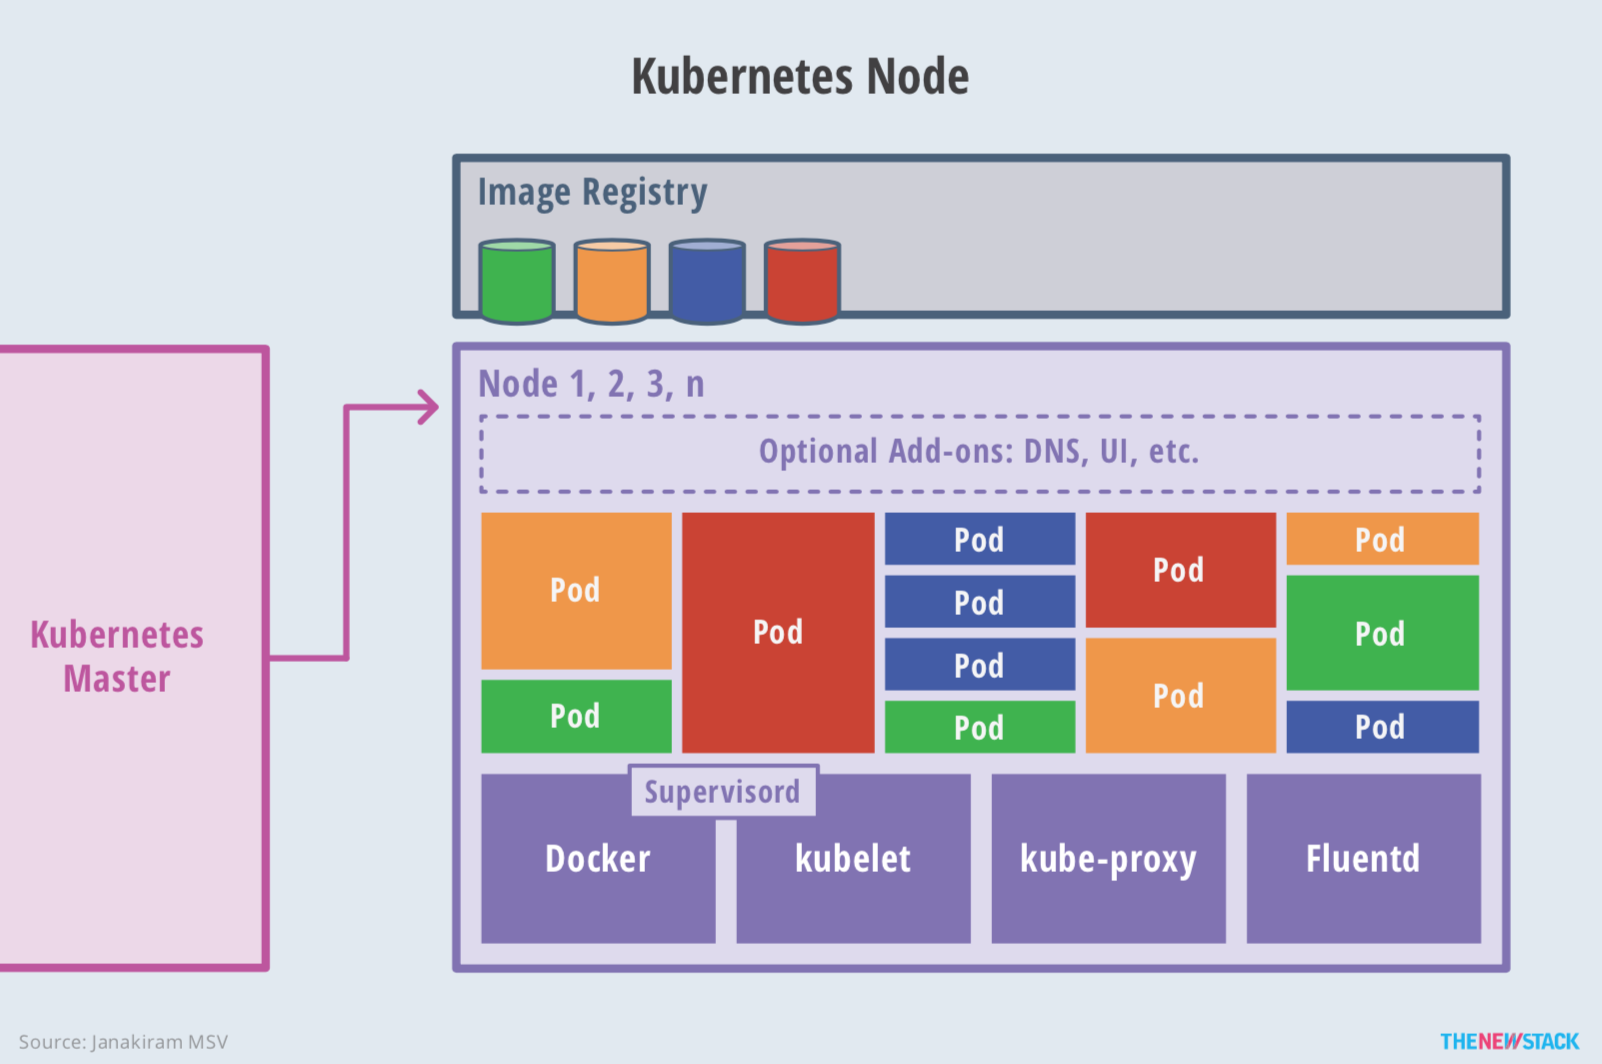
\includegraphics[scale=0.5]{Images/Kubernetes-workers}
  \captionof{figure}{Componenti dei nodi workers}
\end{center}
\chapter{Funzioni}

\chapter{Razionale}
\chapter{Aspetti analitici}
\chapter{Stili architetturali simili o derivati}
\bibliography{Bibliografia}
\end{document}
